\documentclass[12pt, twoside]{article}
\usepackage[utf8]{inputenc}
\usepackage[T1]{fontenc}
\usepackage{lmodern}
\usepackage{ngerman}
\usepackage{amsmath}
\usepackage{amssymb}
\usepackage{array}
% Grafikpaket laden
\usepackage{graphicx}
\setlength{\parindent}{0em} 
\newcommand{\N}{\mathbb{N}}
\newtheorem{Sa}{Satz}[subsection]
\newtheorem{Kor}{Korollar}[subsection]
\newtheorem{Prop}{Proposition}[subsection]
\newtheorem{Def}{Definition}[subsection]
\begin{document}


\section{Kleine Zusammenfassung}
\subsection{Begriffe}
\textit{Permutation:} Die Gesamtheit der möglichen Kombinationen von Elementen einer gegebenen
Menge miteinader\footnote{Es wird hier nichts gezogen}. Berechnet wird diese mit der Fakultät:
$$n!:= \prod_{i=1}^{n}i$$



Definitionen von leeren Summen und Produkten:

$$
\text{leere Summe } \sum_{i=1}^{0}3=0 \text{, leeres Produkt } \prod_{i=1}^{0}3=1
$$

Die Menge der Elemente, aus denen irgendwas oder mit denen irgendwas passiert,
wird im Kurs als $n$-elementige Menge bezeichnet. 

\subsection{Urnenexperimente}
Es gibt eine Urne mit $n$ Kugeln ($n$-elementige Menge) welche durchnummerriert sind. Es werden $k$ Kugeln gezogen.
\subsubsection{Variation mit Wiederholung}

Es wird eine Kugel gezogen. Die Nummer der Kugel wird notiert (in Reihe nacheinander). Die Kugel
wird zurückgelegt. 

Es sind $n, k \in \N$ mit $n=$ Anzahl der Kugeln und $k=$ Anzahl der Ziehungen. Somit gibt es
$$
n^k
$$
verschiedene Möglichkeiten. \\

\textbf{Ein Beispiel:} Seien $n, k \in \N$. $n=3$ Rechnertypen und $k=6$ Arbeitsplätze. Dann gibt es $n^k=3^6=729$ Kombinationen bzw. Möglichkeiten
die Arbeitsplätze mit Rechnern auszustatten. \\

\subsubsection{Variation ohne Wiederholung}

Es wird eine Kugel gezogen. Die Nummer der Kugel wird notiert (in Reihe nacheinander). Die Kugel wird nicht
zurückgelegt.

Es sind $n, k \in \N \text{ mit } n= \text{ Anzahl der Kugeln und } k= \text{ Anzahl der Ziehungen}$. Es gibt 
$$
\prod_{i=0}^{k-1}(n-i)
$$
verschiedene Möglichkeiten.

\textbf{Ein Beispiel:} Seien $n, k \in \N$ mit $k=2=$ Anzahl Zimmer und $n=4=$ Anzahl Farben. Kein Zimmer darf
die Farbe eines anderen Zimers haben. Dann gibt es 
$$
\prod_{i=0}^{2-1}(4-i)=(4-0)\cdot (4-1)=4 \cdot 3 = 12
$$
verschiedene Kombinationen bzw. Möglichkeiten die Zimmer zu streichen ohne dass eine Farbe doppelt verwendet worde (Zimmer 1
grün und Zimmer 2 blau ist hierbei eine andere Kombination als Zimmer 1 blau und Zimmer 2 grün).

\subsubsection{Kombination ohne Wiederholung}
Es wird eine Kugel gezogen. Die Nummer wird notiert. Die Kugel wird nicht zurückgelegt. Die Reihenfolge der Nummern
spielt hier keine Rolle. Somit ist die Kombination \{1, 2\} die Gleiche wie \{2, 1\}. \\

Es sind $k, n \in \N \text{ mit }k= \text{ Anzahl der Ziehungen}$, $X$ die Menge aller Kugeln mit $\{1, 2, 3, \dots, n\}$ und $|X|= \text{Anzahl der Kugeln}=n$. Es gibt 
$$
\binom{n}{k}:= \frac{n(n-1)(n-2) \cdot \ldots \cdot (n-k+1)}{1 \cdot 2 \cdot \ldots \cdot (k-1)k} = \frac { \prod_{i=0}^{k-1}(n-i)}{k!}
$$
verschiedene Kombinationen bzw. Möglichkeiten. \\

\textbf{Ein Beispiel:} Seien $k, n \in \N$ und die Menge Zimmer mit $M:=\{ \text{Raum1, Raum2} \}$, $|M|=2=k$ und $n=4=$ Anzahl Farben. Kein Zimmer darf
die Farbe eines anderen Zimmers haben und jede Kombination darf nur ein mal vorkommen\footnote{ \{rot, grün\} = \{grün, rot\}}. Laut der Formel gibt es
$$
\binom{4}{2}:=\frac { \prod_{i=0}^{2-1}(4-i)}{2!} = \frac{(4-0)(4-1)}{1 \cdot 2}= \frac{12}{2}=6
$$
verschiedene Kombinationen bzw. Möglichkeiten die Zimmer zu streichen, ohne dass eine Farbe doppelt verwendet worde (Zimmer 1
grün und Zimmer 2 blau ist hierbei eine andere Kombination als Zimmer 1 blau und Zimmer 2 grün).






\subsection{Teilmengen}
Gegeben sei eine Menge $X$ mit $X=\{2, 4,22 ,1\}$. Dann ist die Mächtigkeit bzw. Kardinalität von $X=|X|=4$. Die Anzahl der Teilmengen bestimmt
man mit
$$
|2^X|=2^{|X|}=16.
$$
Somit hat $X$ 16 Teilmengen. Die Anzahl der ungeraden\footnote{ungerade Anzahl von Objekten in der Teilmenge} Teilmengen wird mit $2^{|X|-1}$ 
berechnet. Der gerade Anteil hat die selbe Größe. Die Menge $X$ hat somit $2^{4-1}=2^3=8 \text{ gerade und } 8 \text{ ungerade Teilmengen}$.

\subsection{Übersicht}
Für die Anzahl der Möglichkeiten, aus $n$ Objekten $k$ auszuwählen, gilt: \\


\begin{centering}
\begin{tabular}{l||p{4.5cm}|p{4.5cm}}
Auswahl... & \textbf{mit} Beachtung der Reihenfolge (Variation) & \textbf{ohne} Beachtung der Reihenfolge (Kombination) \\
\hline
\hline
\textbf{ohne} Zurücklegen &  $$\binom{n}{k}k!$$  & $$\binom{n}{k}$$  \\
\hline
\textbf{mit} Zurücklegen & $$n^k$$ & $$\binom{n+k-1}{k}$$ \\

\end{tabular}
\end{centering}


\section{Propositionen, Korollare, Sätze}
\begin{Prop} Seien $n, m \in \N, m \ge 1$ und $A$ eine $n$-elementige Menge und $R$ eine $m$-elementige Menge. Dann ist die 
Anzahl aller Abbildungen $f:A \Rightarrow R$ gerade $m^n$.
\end{Prop}
\begin{Kor} 
Sei $X$ eine $n$-elementige Menge, $n \in \N$. Dann hat $X$ genau $2^n$ Teilmengen, oder als Formel
\end{Kor}
$$|2^X|=2^{|X|}$$





\begin{Prop} Sei  $n \ge 1$. Jede n-elementige Menge hat genau $2^{(n-1)}$ Teilmengen mit ungerade vielen Elementen und 
ebenso viele mit gerade vielen Elementen. 
\end{Prop}

\begin{Prop} Seien $m, n \in \N $. Dann gibt es genau 
$$
m(m-1)\dots (m-n+1)= \prod_{i=0}^{n-1} (m-i)
$$
injektive Abbildungen einer gegebenen n-elementigen Menge A in eine gegebene m-elementige Menge R.
\end{Prop}

\begin{Def} Sei $n \in \N$. Die Zahl
$$
n!:= \prod_{i=1}^{n}i=1c\cdot 2 \cdot \ldots \cdot(n-1)\cdot n
$$
nennen wir die Fakultät von $n$.
\end{Def}

Es gibt eine Menge die auf sich selber abbildet. Zum Beispiel die natürlichen Zahlen 1-7 bilden auf die natürlichen Zahlen 1-7 
bilden die Menge M, die auf sich selbst abbildet. 1 auf 4, 2  auf 7, 3 auf 5, 4 auf 1, 5 auf 2, 6 auf 3 und 7 auf 5. Diese „Mischung“ 
nennt sich Permutation.  Es gibt verschiedene Möglichkeiten zu Mischen, verschiedene Permutationen. Die Möglichkeiten kann man mit Fakultät bestimmen. 
Die Mächtigkeit der Menge, also |M| als Fakultät.

\begin{Prop} 
Jede Permutation $\sigma$ lässt sich (bis auf die Reihenfolge eindeutig) in paarweisen disjunkten Zyklen zerlegen.
\end{Prop}

\begin{Sa}[Binomischer Satz]
Sei $n \in \N$. Dann ist
$$
(1+x)^n= \sum_{k=0}^{n} \binom{n}{k}x^k.
$$
\end{Sa}

\begin{Kor}
$$
(a+b)^n= \sum_{k=0}^{n} \binom{n}{k}a^kb^{n-k}.
$$
\end{Kor}


\begin{Kor}
$$
\binom{n}{0}+\binom{n}{1}+\binom{n}{2}+\cdots+\binom{n}{n}=2^n.
$$
\end{Kor}

\begin{Prop}
$$
\sum_{i=0}^{n}\binom{n}{i}^2=\binom{2n}{n}.
$$
\end{Prop}

\subsection{Fragestellung - Multinomialkoeffizient}
Wieviele Zeichenketten kann man aus den Buchstaben des Wortes BANANE bilden? Man kann aus 
6 Buchstaben 6! verschiedene Anordnungen (=720) bilden. Dabei wird aber jedes  Wort 4 mal vorhanden sein,
 da die Buchstaben $N$ und $A$ je zweimal vorkommen. Die Anzahl der Möglichkeiten ist also 
 $\frac{6!}{1! 2! 2! 1!}=180$. \begin{Def} Sei $k_1+ \ldots + k_m = n$. Der Multinomialkoeffizient ist definiert als
$$
\binom{n}{k_1, k_2, \ldots, k_m}:=\frac{n!}{k_1 k_2! \ldots k_m!}.
$$

\end{Def}

Der Multinomialkoeffizient beschreibt also die Anzahl der Möglichkeiten, $n$ Objekte, von denen jeweils
$k_i$ nicht unterscheidbar sind, anzuordnen. Im Falle $m=2$ erhalten wir wieder den Binomialkoeffizienten.

$\binom{n}{k}$ und der Binomialsatz haben dann folgende Verallgemeinerungen:


\begin{Sa}[Multinomialsatz]. Sei $n \in \N$. Dann ist
$$
\sum_{\substack{i=1 \\ k_i\ge1}}^{m}\binom{n-1}{k_1, \dots, k_{i-1}, k_i-1, k_{i+1}, \dots, k_m} = \binom{n}{k_1, \dots, k_m}, 
$$
$$
(x_1+x_2+ \ldots +x_m)^n = \sum_{\substack{k_1+\ldots+k_m=n \\ k_1, \dots, k_m\ge0}} \binom{n}{k_1, k_2, \dots, k_m}x_1^{k_1} x_2^{k_2} \ldots x_m^{k_m} .
$$
\end{Sa}



\begin{figure}
	\centering
	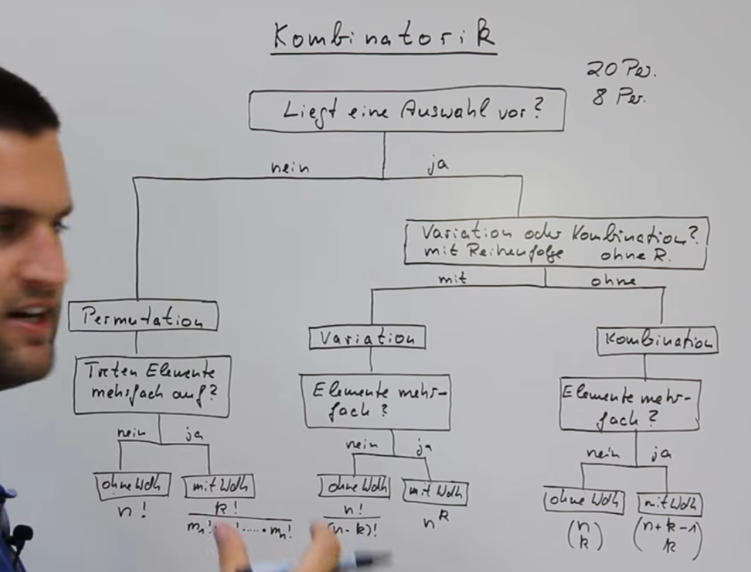
\includegraphics[height=12cm]{bld1.png}
	\caption{Übersicht Kombinatorik}
	\label{img:grafik-dummy}
\end{figure}
\end{document}
\grid

